\documentclass[letter,openright,12pt,spanish]{report}
%Gummi|065|=)
\title{\textbf{Describir las condiciones de singularidad de manipuladores seriales.}}
\author{Mario Alcala Villagomez\\
		Cinem\'atica de Robots\\
		Ing. Mecatronica 7A}
\date{01 de octubre de 2019}
\usepackage{amsmath}
\usepackage{graphicx}
\begin{document}

\maketitle

\section{Introducci\'on}

Los robots paralelos pueden adoptar configuraciones en las cuales las fuerzas articulares no puedan equilibrar los esfuerzos sobre la plataforma m\'ovil. Es importante determinar estas configuraciones en cuya vecindad las fuerzas articulares tienden a infinito y el robot puede colapsar. Un estudio anal\'itico elemental de este tipo de singularidades se puede encontrar en Gosselin y \'Angeles, donde se denominan como 'singularidades de segundo tipo'. Estas disposiciones singulares est\'an caracterizadas por la anulaci\'on del determinante de la matriz jacobiana inversa. A pesar de que esta matriz sea conocida, en la mayor\'ia de los casos la computaci\'on simb\'olica de este determinante no conduce a soluciones anal\'iticas, por lo que hay que recurrir a procedimientos num\'ericos como los propuestos por DOuady. Merlet, hizo un extenso uso de la geometr\'ia de Grassman para enumerar con detalle las condiciones geometr\'icas singulares de diferentes robots paralelos. Liu, realizo un estudio geom\'etrico de las singularidades de la plataforma de Stewar, en el que analizaron la matriz jacobiana para cuatro posiciones singulares. Ma. y \'Angeles, mostraron que algunas arquitecturas sim\'etricas de la plataforma de Stewar, presentan singularidades extendidas por todo el espacio del trabajo o regiones importantes dentro del mismo, caracterizadas por las capacidad de movimiento continuo de la plataforma m\'ovil con todos los actuadores bloqueados. A estas singularidades las llamaron singularidades de arquitectura. AUnque estas singularidades dan lugar a serios problemas de control, \'estas se pueden eliminar en la fase del diseño, Gosselon estudi\'o la asociaci\'on del condicionamiento de la matriz de transformaci\'on est\'atica con la rigidez de la plataforma de Stewar, donde se perd\'ia rigidez cerca de configuraciones singulares. Un problema que queda por resolver es determinar de forma simult\'anea si existen configuraciones singulares  dentro del espacio de trabajo de un robot, Sefrioui Bhattacharya, desarrollo un esquema de planificaci\'on de trayectorias evitando singularidades, de forma que reestructuraba la planificaci\'on en la vecindad de una singularidad. Luego Dasgupta y Mruthynjaya, formularon el problema de la planificaci\'on de la planificaci\\on de trayectorias evitando singularidades y desarrollaron una estrategia para planificar entre dos puntos trayectorias bien condicionadas en el espacio de trabajo del robot.

\section{Singularidades del manipulador}

Los valores de \textit{q} que hacen singular una matriz Jacobiana se conoce como puntos singulares. En ellos la perdida de un grado de libertad que el manipulador realice desplazamientos en un determinado sentido. Es m\'as, matem\'aticamente, el movimiento cartesiano en el sentido de la singularidad conllevaria una velocidad infinita en el espacio articular en alguna de sus variables articulares.\\
Resumidamente:\\

En las inmediaciones de las configuraciones singulares, un movimiento a velocidad constante en el espacio cartesiano del extremo del robot, obligatoria a movimientos de las articulaciones m\'as rapidos en la medida en que m\'as cerca se encuentre de la configuraci\'on singular volvi\'endose inabordables por el sistema de actuaci\'on.\\

Las singularidades representan configuraciones en las que la movibilidad de la esctructura se reduce, es decir, no es posible imponer un movimiento arbitariio (de los habitualmente posibles) al efector final.\\

Las diferentes singularidades del robot se puede clasificar en dos tipos:\\

Singularidades de contorno: Se presentan cuando el extremo del robot est\'a en alg\'un punto del limite del espacio de trabajo interior exterior. Estas configuraciones por su propia naturaleza no son especialmente peligrosas ya que son evitables no llevando el manipulador a las zonas extremas del espacio de trabajo alcanzable.\\

Singularidades internas: Se producen en el interior del espacio de trabajo alcanzable y son generalmente causadas por la alineaci\'on o m\'as articulaciones del robot.\\

\subsection{Ejemplo}

Un ejemplo de singularidad de contorno se puede ver en la figura siguiente en donde el robot Puma extendido es incapaz de moverse tanto hacia el exterior o el interior de la flecha roja. De forma an\'aloga la figura de la derecha representan una singularidad interna, en donde si se intenta desplazar el extremo del robot en cualquier direcci\'on con componente perpendicular al plano formado por la segunda y tercera articulaci\'on, se obligar\'a a la primera articulaci\'on a realizar un grio a velocidad infinita:\\

\begin{figure}[htp]
\centering
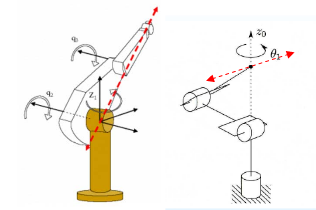
\includegraphics[width=8cm]{/home/sarha13/Escritorio/01.png}
\caption{Robot Puma}
\label{Figura 1}
\end{figure}
Uno de los casos m\'as cl\'asicos en robots de seis grados de libertad se producen cuando hay una alineaci\'on de ejes de orientaci\'on de la mu\~neca, normalmente el 4to con el 6to.\\ 
Para obtener matem\'atematicamente los puntos de singularidad del robot, como se ha visto, es suficiente con plantear la ecuaci\'on:

\begin{displaymath}
det(f(q)=0)
\end{displaymath}

Obviamente analiticamente esta es una operaci\'on ciertamente compleja.

\section{Desacoplo de la Jacobiana}

Debido a la alta complejidad de c\'alculo que requiere el c\'omputo de las singularidades, se divide el problema en dos: Hallar las singularidades del brazo rob\'otico por un lado y hallar las sssingularidades de orientaci\'on del extermo operativo por otro. Es decir, se en vez de utilizar como sistema de referencia del extremo el extremo operativo, se utiliza el punto de mu\~neca, la matriz Jacobiana resultante, trat\'andose del mismo mecanismo, es triangular infierior por cajas. Es decir, sea $\textit{J}_m$(q) la matriz jacobiana del sistema de refrencia que localiza el punto de mu\~neca -su posici\'on no es afectada por las tres \'ultimas articulaciones aunque si su orientaci\'on-, entonces:

\begin{displaymath}
J_m(q)=[
\begin{matrix}
	J_{11_{2x2}} & 0_{3x3}\\
	J_{21_{2x2}} & j_{22_{2x23}}\\
\end{matrix}
]\Longrightarrow det (J_m)=det(J_{11})def(J_{22})
\end{displaymath} 
y por tanto el resultado de analizar el primer determinante $det(J_{22})=0$ se denomina como \textbf{singularidades de brazo}, mientras que el an\'alisis $det(J_{22})=0$ tendr\'a como resultado lo que se den\'omina como \textbf{singularidades de mu\~neca}.

\section{Signularidades}

Las configuraciones singulares de un amnipulador paralelo ocurren cuando al menos una de las dos matrices Jacobianas es singular. Se tienen los siguientes casos:\\
Si \textbf{A} es singular, se dice que el manipulador est\'a bajo una \textit{configuraci\'on singular paralela}. Gana g.d.l(grado de libertad).\\
Si \textbf{B} es singular, se dice que el manipulador est\'a bajo una \textit{configuraci\'on singular serial}. Pierde g.d.l\\
Si \textbf{A} y \textbf{B} son singulares.

\begin{figure}[htp]
\centering
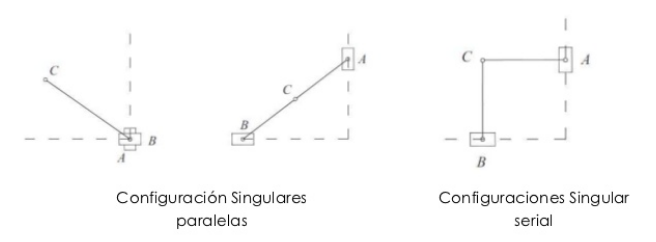
\includegraphics[width=7cm]{/home/sarha13/Escritorio/02.png}
\caption{Configuraci\'on para un manipulador 2RRR}
\label{Figura 2}
\end{figure}

\begin{figure}[htp]
\centering
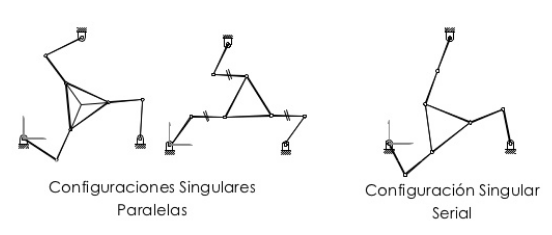
\includegraphics[width=7cm]{/home/sarha13/Escritorio/03.png}
\caption{Configuraci\'on de un amnipualdor 3RRR}
\label{Figura 3.}
\end{figure}
\end{document}
